% !TEX TS-program = xelatex
% !TEX encoding = UTF-8

% This is a simple template for a XeLaTeX document using the "article" class,
% with the fontspec package to easily select fonts.

\documentclass[11pt]{article} % use larger type; default would be 10pt

\usepackage{fontspec} % Font selection for XeLaTeX; see fontspec.pdf for documentation
\defaultfontfeatures{Mapping=tex-text} % to support TeX conventions like ``---''
\usepackage{xunicode} % Unicode support for LaTeX character names (accents, European chars, etc)
\usepackage{xltxtra} % Extra customizations for XeLaTeX
\usepackage{float}
%\setsansfont{Deja Vu Sans}
%\setmonofont{Deja Vu Mono}

% other LaTeX packages.....
\usepackage{geometry} % See geometry.pdf to learn the layout options. There are lots.
\geometry{a4paper} % or letterpaper (US) or a5paper or....
%\usepackage[parfill]{parskip} % Activate to begin paragraphs with an empty line rather than an indent

\usepackage{graphicx} % support the \includegraphics command and options

\title{Environnement du travail}
\author{Moncef BEN RAJEB}
%\date{} % Activate to display a given date or no date (if empty),
         % otherwise the current date is printed 

\begin{document}
\maketitle
\section{Introduction}
\paragraph{}
Certes, le sucées ou l'échec d'un projet informatique dépend du choix des technologies utilisés.
Ce choix dérive essentiellement des objectifs à attendre et des contraintes d'accompagnement qui doivent être prisent en considération.
\paragraph{}
Dans cette partie je vais présenter les différentes technologies envisageables par les architectes de Stample 
et relatives à la développement du Backend la partie sur la quel j'ai travaillé et le FrontEnd.
Vous trouverez plus de détailles sur l'environnement du travail sur ma page\footnote{http://ideas2d.com/moncef/home.php} web.
\section{Working tools}
\subsection{Environnement de Développement}
\begin{itemize}
\item PlayFramework\footnote{http://www.playframework.com/} 2.1.0
\item JDK 7
\item Maven3
\item OS X 10.8.4
\item SBT\footnote{http://www.scala-sbt.org/} 0.12.4
\item ElasticSearch\footnote{http://www.elasticsearch.org/} 19.4.0
\item MongoDB\footnote{http://www.mongodb.org/} 2.2.x

\end{itemize}

\subsection{Langages de Programmation}
\begin{itemize}

\item BackEnd : SCALA , JAVA, JSON
\item FrontEnd : HTML5, JavaScript, Jquery, CSS3, JSON, Ajax. 

\end{itemize}
\subsection{Plugins}
\begin{itemize}

\item BackEnd : SecureSocial, Salat,
\item FrontEnd :Backbonejs 

\end{itemize}
\subsection{Outils de développement}
\begin{itemize}
\item IDE : ItelliJ IDEA 12.1.14 Community Edition;
\item Base de donnée : Mongodb NoSQL data base;
\item outils de compilation automatique : sbt.
\end{itemize}
\section{Aspects technique de Stample}
\subsection{Architecture}
\begin{figure}[H]
        \centering
                \centering
                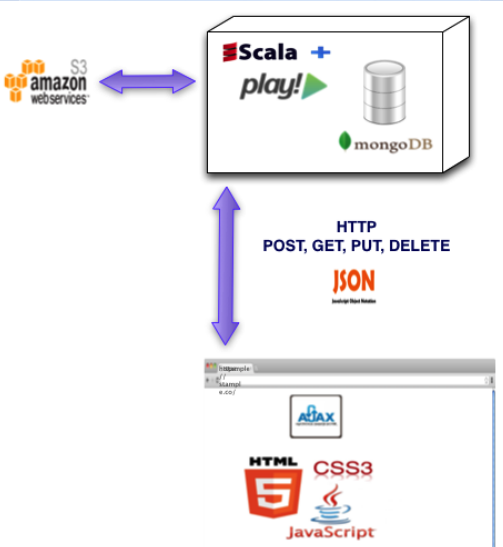
\includegraphics[width=10cm,height=8cm]{architectureStample.png}
                \caption{Architecture de la plateforme}
                \label{fig:Architecture de la plateforme}
       
\end{figure}
\subsection{Description de l'architecture globale}
\paragraph{}
Les requêtes HTTP sont faites en JSON.
Le JSON est désérialisé dans des objets métiers 
(Scala case class) pour être manipulés au sein de l'application.
\subsubsection{Communication entre la base et l'API}
\paragraph{}
On utilise le driver Casbah MongoDB en Scala et une librairie "Salat" qui permet une bonne intégration de Casbah dans l'application.
Salat permet de sérialiser les objets métiers (case class) en BSON \footnote{http://bsonspec.org/}, cette libairie propose un DAO (Data Access Object) générique un model companion qui expose les méthodes basique des requêtes Mongo (find(), findById(), search()...)
\subsubsection{Communication entre L'API et ElasticSearch}
\paragraph{}
L'indexation dans la base se fait manuellement après l'insertion, la mise à jour d'un document MongoDB dans la base de donnée.
L'échec d'indexation est non bloquant car il est ratrappé par un Job.
\paragraph{}
ElasticSearch prend en entrée du JSON cela implique qu'il fontionne particuliérement bien avec Mongo.
De plus, utilise salat aussi pour produire le JSON d'un objet métier (case class).
Donc nous avons le même document dans MongoDB et ElasticSearch. Cela permet de rendre un document similaire à Backbone pour la recherche.
On utlise un client JAVA pour ElasticSearch.
\subsubsection{SBT}
\paragraph{}
Le build est réalisé par SBT, il faudrait mettre en place un Jenkins qui fera tourner les tests unitaires et embarqués à chaque push pour réparer les regressions et que nous en soyons alertés.
\subsubsection{Les collections MongoDB}
\paragraph{}
Stample structure les données sous forme de diffirents collections.
Ils Sont tous identifier par un ObjectId, elle regroupe tout les informations nécessaire sur les utilisateurs (Compte utilisateurs, Stamples ...).
\subsection{Configuration de départ}
\subsubsection{Description de la configuration}
\paragraph{}
Le projet contient de quatre répertoires séparer : fixturedatabase contenant les fichiers JSON et leurs sérialisation binaire encodé BSON, restore inclu le build de l'application et les plugins, stample-search contenant les classes java et la configuration nécessaire pour le lancement du projet et stample-web contient les diffirents packages du Front/back End.
\paragraph{}
Pour l'interraction avec le projet le permier pas est l'installation des outils cités auparavant. ensuite, j'ai configuré ma machine avec les paths nécessaires pour lancer sbt, play, mongo et elasticSearch. Puis, j'ai lancé le mvn dans le repartoire stample-search. Enfin il est indisponsable de lancer play ou sbt et de générer les fichier idea, eclipse ou autre dans stample-web avec l'IDE envisagé.     
\subsubsection{Gestion du travaille en groupe}
\paragraph{}
Les régles du travaille en groupe sur le projet :
\begin{enumerate}
\item NE PAS travailler directement sur la branche master. Ce n'est que pour la production.
\item La branche de développement principale est "preProd". A partir de cette branche on commence une nouvelle branche. 
\item Lors du développement sur une branche, merger régulièrement preProd en elle, pour s'assurer d'être à jour avec le travaille des autres développeurs.
\item Lorsque la branche est stable et a été testé par le chef de projet, il va tester, merger dans preProd, puis on peut supprimer cette branche.
\item Utiliser toujours camelCase pour nommer les branches et des noms intelligents!
\item Ajouter des explications intelligents lors de chaque commit.

\end{enumerate}
\section{Conclusion}
\paragraph{}
Dans cette partie j'ai détaillé les outils qu'on utilises. Ensuite, j'ai présenté l'architécture globale de la plateforme et les diffirentes interractions. La prochaine section se focalise sur la solution développer pour le login sur Stample.


\end{document}